\documentclass[12pt]{article}
\usepackage[margin=1in]{geometry}
\usepackage[pdftex]{graphicx}
\usepackage{multirow}
\usepackage{setspace}
\usepackage{enumitem}
\pagestyle{plain}

\begin{document}

\noindent
% Course information
\begin{tabular*}{\textwidth}{l @{\extracolsep{\fill}} r}
  & \multirow{3}{*}{
\includegraphics[height=1.0in]{logo.jpg}} \\
  \large Introduction to Physics Computation & \\
  \large Fall Quarter 2021 & \\
  \large Physics 40 & \\
\end{tabular*}
\vspace{10mm}

\noindent
% Professor information
\begin{tabular}{ l l }
  \multirow{6}{*}{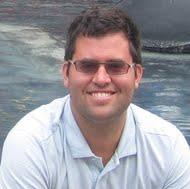
\includegraphics[height=1.25in]{mike.jpg}} & \\
  & \\
  & \large Michael Mulhearn \\
  & \large mulhearn@physics.ucdavis.edu \\
  & \large Physics 317 \\
  & \\
\end{tabular}
\vskip 0.5cm
\noindent
\textbf {Lectures:} M,W 3:10-4:30 PM in Kerr 293
\begin{tabbing}
\hspace*{3em}\= \hspace*{5em} \= \kill % set the tabbings
\textbf {Lab:}    \> Section 1: \> T,H 3:10-5:00 PM (TBA)
\end{tabbing}
\noindent
\textbf {Text:}\\
Online lecture notes at {\tt https://www.scipy-lectures.org}\\
Lab Manual available on course website\\
Gezerlis ``Numerical Methods in Physics with Python'' is available online at the UC Davis library.\\
% Garcia?

\noindent
\textbf{Office Hours:} TBD \\

\noindent
\textbf{Lab Instructor:} Keerthi Vasan (kvch@ucdavis.edu) \\

\noindent
\textbf {Course Description:}  
Introduction to programming with examples from numerical analysis and
computational physics. Introduction to modern tools used for
scientific analysis and computer algebra.\\

\noindent
\textbf{Lectures:} The primary emphasis of this course will be on
learning by doing.  The purpose of the lecture is to prepare you for
the lab activities.  The lectures will be a mix of traditional board
lecture and projected live computing.\\

\noindent
\textbf{Quizzes:} Starting in Week 2, there will be a short low-stakes
quiz at the start of each Wednesday lecture.  Generally, it will be in
the form a Parsons Problem: you will select and order provided code
fragments to achieve a state objective.\\

\noindent
\textbf{Interviews:} Each week I will select a subset of students for
a brief interview during the Thursday lab section. \\

\noindent
\textbf {Jupyter Notebooks:}\\ 
The lab manual describes numerical problems which you should complete
with Scientific Python in Jupyter Notebooks.  Even though you may work
together, each student must maintain their own notebook for each lab.

Start each of your notebooks with the magic python function
{\tt\%pylab inline} to load numpy as np, matplotlib as plt, and show
plots as cell output (inline).  Make sure all of your output is
visible, print your notebook as a PDF file, and post the PDF file to
the course web site by Friday evening.\\

\noindent
\textbf {Pencil and Paper:}\\ 
Occassionally, the lab manual will include some pencil and paper computations.  You should take a picture of your pencil and paper, or scan to PDF, and submit to the course website along with your Jupyter Notebook.\\

\noindent
\textbf {Reinventing the Wheel:}\\
There are many exercises in this course which involve implementing
software that is likely already available elsewhere.  This approach
is usually a bad idea.  It is a programming {\em anti-pattern} called
``Reinventing the Wheel''.  Generally one should use library functions
instead of homemade solutions whenever possible, as the library
versions are thoroughly debugged.  In this case, however, we are doing
this deliberately as an exercise.  Even when you are quite experienced
at programming, you will sometimes opt to re-implement something as a
learning experince, just as we are doing here.  The anti-pattern would
be to continue using the homebrew solution after the learning
experience instead of a superior existing solution.

You may use the internet to search for solutions to specific technical
challenges, but you {\em may not} search for top-level solutions to
the assignments.  So ``how to use a while loop in Python'' is
perfectly fine but ``how to sum fractions in Python'' is not.  The
interviews and quizes are designed to check that you understand the
completed exercises at a level that would be difficult to reach with
cut-and-paste.

\noindent
\textbf{Final Grades:} The final grades will be based on a weighted
average of the submitted lab exercises, quizzes, interviews, and lab
attendance. \\

\noindent
\textbf{Daily Symptom Survey:}\\
You must complete the daily symptom survey to attend any in-person
activities.  If you fail your daily symptom survey, forward the
results to your instructor and follow the instructions under unable to
attend activity.

\noindent
\textbf{Inability to Attend:}\\
If you are unable to attend an activity, you may immediately request the following accommodations:
\begin{itemize}
  \item 





Failing the delay symptom survey will excuse you from up to two quizes, allow you to This will grant you permission to
attend the lab section remotely.





quarantine status, by e-mail,
to your instructor.  The accommodations which will be made during a
verified quarantine include: (1) permission to connect to lab sections
remotely, (2) excused from quizes, (3) rescheduled interviews (4)
opportunity to review missed lecture material during office hours.

There is no option to take exams remotely.  If you cannot attend an
exam due to quarantine or sickness, you may request an Incomplete and
take the a make-up exam at a future date.  This option will only be
available to students who have completed their other assignments at
the passing level.

\newpage

\noindent
\textbf {Course Schedule}:\\
Note that the dates refer to lectures.  The lab date is the next day.
The topics and schedule may be adjusted while the course is in
progress.\\


\begin{table}[h!]
\normalsize % The size of the table text can be changed depending on content. Remove if desired.
\begin{tabular}{ lll }
\hline
\textbf{Week} & \textbf{Lab Date} & \textbf{Lab} \\
\hline
1  & 22 Sep & Installation \\
\hline
2  & 27 Sep & Binary Numbers \\
   & 29 Sep & Sequences and Series \\
\hline
3  & 4 Oct  & TBD \\
   & 6 Oct  & TBD \\
\hline
4  & 11 Oct & TBD \\
   & 13 Oct & TBD \\
\hline
5  & 18 Oct & TBD \\
   & 20 Oct & TBD \\
\hline
6  & 25 Oct & TBD \\
   & 28 Oct & TBD \\
\hline
7  & 1 Nov  & TBD \\
   & 3 Nov  & TBD \\
\hline
8  & 8 Nov  & TBD \\
   & 10 Nov & TBD \\
\hline
9  & 15 Nov & TBD \\
   & 17 Nov & TBD \\
\hline
10 & 22 Nov & TBD \\
   & 24 Nov & (Cancelled)\\
\hline
11 & 29 Nov & TBD \\
   & 1 Dec  & TBD \\
\hline
\end{tabular} 
\end{table}

\end{document}

